% Template for ICME 2020 paper; to be used with:
%          spconf.sty  - ICASSP/ICIP/ICME LaTeX style file, and
%          IEEEbib.bst - IEEE bibliography style file.
% --------------------------------------------------------------------------
\documentclass{article}
\usepackage{spconf,amsmath,epsfig}
\usepackage{url}
\usepackage{tikz}

\usetikzlibrary{shapes.geometric, arrows}

\let\OLDthebibliography\thebibliography
\renewcommand\thebibliography[1]{
  \OLDthebibliography{#1}
  \setlength{\parskip}{0pt}
  \setlength{\itemsep}{0pt plus 0.3ex}
}

\pagestyle{empty}


\begin{document}\sloppy

% Example definitions.
% --------------------
\def\x{{\mathbf x}}
\def\L{{\cal L}}


% Title.
\title{A Machine Learning Approach For Fast CU Partitioning And Time Complexity Reduction in Video Coding}


\name{Md. Zahirul Islam$^{\#}$, Md. Eimran Hossain Eimon$^{\#}$, Boshir Ahmed$^{\#}$}
\address{$^{\#}$Rajshahi University of Engineering \& Technology, Rajshahi,  Bangladesh}

\maketitle


\begin{abstract}

Modern video codecs such as HEVC have high capability to minimize the bits and also have an immense complexity because of testing more combinations during the RDO (Rate Distortion Optimization) process. Partitioning a coding unit (CU) into smaller ones is the leading cause of the increased time complexity. For this reason, we need a fast and efficient algorithm for real-time applications. In this paper, we proposed an approach for reducing the time complexity of CU splitting by using decision tree classifier. By using the proposed method, it is possible to skip a block if the block contains only a single motion, i.e. if the block falls in a homogeneous region. Experimental results show that on average 45.02\% time complexity reduction is possible by implementing the skip criterion. However, as a trade-off on average 1.38\% bit rate is increased over standalone HEVC.

\end{abstract}

\begin{keywords}
 Video Coding, Complexity Reduction, Motion Discontinuity, Machine Learning, Decision Tree.
\end{keywords}


\section{Introduction}
\label{sec:Introduction}


A natural video has multiple objects and each object has different shapes or boundaries, depths, illumination and texture. Typical video scene has both spatial and temporal characteristics. Spatial category includes the number of objects and shapes, color and texture variation in the scene; whereas the temporal category includes camera motion, objects movement and illumination change. If a coding unit contains multiple motions such as camera motion, movement of the objects or object boundaries then further partitioning is occurred in the traditional video codecs during the RDO process. Containing multiple motions in a block is defined as Motion Discontinuity in this paper. On the other hand, if a CU contains only a single motion, i.e. the CU falls in a uniform or homogeneous region then there is no need to split this CU again. \\

\begin{figure}[t]
	\centering
	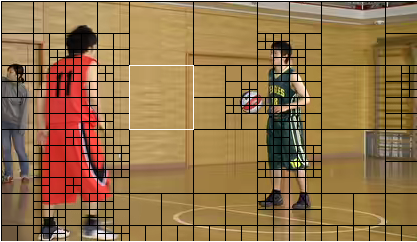
\includegraphics[width=3in, height= 1.5in]{Figures/elecard_partitioning}
	\caption{An example of CTU (Coding Tree Unit) partitioning scheme by the permission of elecard software. White boundary block is an example of homogeneous region. }
	%\vspace{-2.5mm}
	\label{fig:elecard_partitioning}
\end{figure}
\begin{figure}
	\centering
	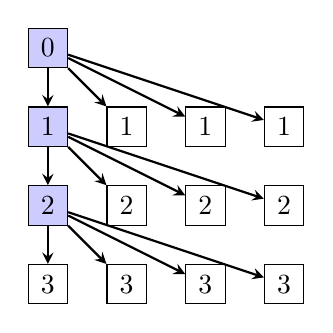
\begin{tikzpicture}[node distance=1cm]
	\tikzstyle{process} = [rectangle, minimum width=0.5cm, minimum height=0.5cm,text centered, draw=black, fill=white!100]
	\tikzstyle{process1} = [rectangle, minimum width=0.5cm, minimum height=0.5cm,text centered, draw=black, fill=blue!20]
	\tikzstyle{arrow} = [thick,->,>=stealth]
	\node (pro1) [process1] {{0}};
	\node (pro2) [process1, below of = pro1] {{1}};
	\node (pro3) [process, right of = pro2] {{1}};
	\node (pro4) [process, right of = pro3] {{1}};
	\node (pro5) [process, right of = pro4] {{1}};	
	\node (pro6) [process1, below of = pro2] {{2}};
	\node (pro7) [process, right of = pro6] {{2}};
	\node (pro8) [process, right of = pro7] {{2}};
	\node (pro9) [process, right of = pro8] {{2}};	
	\node (pro10) [process, below of = pro6] {{3}};
	\node (pro11) [process, right of = pro10] {{3}};
	\node (pro12) [process, right of = pro11] {{3}};
	\node (pro13) [process, right of = pro12] {{3}};
	
	\draw [arrow] (pro1) -- (pro2);
	\draw [arrow] (pro1) -- (pro3);
	\draw [arrow] (pro1) -- (pro4);
	\draw [arrow] (pro1) -- (pro5);	
	\draw [arrow] (pro2) -- (pro6);
	\draw [arrow] (pro2) -- (pro7);
	\draw [arrow] (pro2) -- (pro8);
	\draw [arrow] (pro2) -- (pro9);	
	\draw [arrow] (pro6) -- (pro10);
	\draw [arrow] (pro6) -- (pro11);
	\draw [arrow] (pro6) -- (pro12);
	\draw [arrow] (pro6) -- (pro13);
	\end{tikzpicture}
	\caption{A quad-tree partitioning structure with corresponding depth. 0 marked block size is 64 $\times$ 64 and corresponding depth is 0 (root node), all 1 marked block size is 32 $\times$ 32 and corresponding depth is 1, all 2 marked block size is 16 $\times$ 16 and corresponding depth is 2, all 3 marked block size is 8 $\times$ 8 and corresponding depth is 3 (leaf node).}
	\label{fig:CTU_partitioning}
	\vspace{-5.5mm}
\end{figure}


Modern video coding standards such as HEVC \cite{H.265} and AV1 \cite{AV1} have high efficiency of bit reduction and increased time complexity compared to its previous standards or predecessors like AVC. The high efficiency of modern codecs, including VVC is achieved by having the capability of flexible partitioning so-called coding quad-tree \cite{kim2012block}. For example, HEVC partitions the CUs, which are containing multiple motions for the reduction of bits. This concept can be said in another way: a region with relative motions or object boundaries needs more bits for describing it and needs partitioning. The opposite is true for the region with no motions or no object boundaries, i.e. containing single motion (uniform region), and this paradigm is illustrated in fig. \ref{fig:elecard_partitioning}. A CU partitioning scheme is shown in fig. \ref{fig:CTU_partitioning}, where partitioning occurs in-depth 0, 1 and 2 that's are represented by mid-gray marked block respectively \cite{H.265}. To decide a CU is split or not, the cost function of rate-distortion optimization (RDO) is examined for all possible combinations and this optimization loop is continued until the optimal values are found that optimize J for a given $\lambda$ in equation \ref{eqn_example:RD}. The Lagrange rate-distortion cost function is given below:

\begin{equation}
\label{eqn_example:RD}
\min_{m} J(m) = D(m) + \lambda . R(m)
\end{equation}

Here, $\lambda$ is the Lagrange multiplier, m $\in$ M, M is the set of all possible parameter combinations, R is the rate, D is the distortion which is commonly known as the sum of squared errors and J is the rate-distortion (RD) cost. The complexity of RDO process totally, depends on M and there are more than 75,000 parameter combinations are possible for a root level coding unit (64 $\times$ 64). \\

To reduce the time complexity in encoder side, many guidelines are suggested in different ways. A similar group of research is already proposed to minimize the coding units complexity by using smart-based conditions \cite{vanne2014efficient,heindel2015fast}. Skipping some mode tests of individual nodes (CUs), at the time of RDO process is a way to speed up the encoder. These procedure is known as a fast CU splitting process and this type of research \cite{choi2011coding, gweon2012early, yang2011early} is already included in HEVC reference software. Another way to speed up the encoder by using machine learning approach and this approach has succeeded in most of the cases. Heindel et al. \cite{heindel2016fast} and Zhang et al. \cite{zhang2015machine} proposed a fast CU split decision by using SVM (Support Vector Machine) classifier. Heindel showed that 60\% time complexity is saved on average, whereas 3-4\% bit rate is increased by using SVMs for fast splitting the CUs in \cite{heindel2016fast}. A similar study is experimented by Westerland, and they used the decision tree (D-Tree) classifier instead of SVM. This study is very recent and effective for the reduction of complexity. Westerland et al. \cite{westland2019decision} showed that 0.7\% bit rate is increased, whereas 42.1\% encoding time is reduced. The success of the authors of these papers by using machine learning approaches motivated us in this research area. \\

In this paper, we presented a method for splitting a CU or not at the time of rate-distortion optimization (RDO) process. Our model uses the decision tree classifier for classification purpose. The authors of \cite{westland2019decision} also uses decision tree but different features. Our model uses only two features and has a high accuracy for predicting the blocks or CUs where the uniform motion has or not and traditionally as less as features, needs a short time for classification. All two features of a CU are collected before the RDO process is started. If our model has a prediction that a CU has only a single motion, then this CU is skipped for further partitioning and RDO process is early terminated, otherwise this CU is handover-ed to HEVC for further partitioning. In this way. the time complexity is saved. Latest video codec such as versatile video coding (VVC) which is finalized recently, has no such fast split decision as HEVC environment is used there.\\ 

\vspace{-4mm}
The rest of the paper is organized as follows: in section \ref{sec:Dataset Generation}, we explain how the dataset is generated for classification purpose. In section \ref{sec:Classification Process}, classification process is delineated in briefly. We show the experimental results in section \ref{sec:Experimental Analysis}. Finally, the paper is concluded in section \ref{sec:Conclusion}.

%\section{Motion Discontinuity or Background}
%\label{sec:Motion Discontinuity or Background}



\section{Dataset Generation}
\label{sec:Dataset Generation}

In the case of machine learning algorithm, it needs lots of data for training and testing to make a prediction model. Luckily there is a lot of data which are available in the various test video sequences. In the following subsection, how the dataset is formed is described in details.

\subsection{Feature Engineering}
\label{subsec:Feature Engineering}
Features (commonly known as attributes) are used for classification purposes and feature engineering or feature selection is an essential part for designing any kind of machine learning approach. The features are generated from the displayed frame image in this research as the residual image is available in encoder side. Displayed frame difference (DFD) or residual image can be determined by subtracting the motion-compensated prediction frame from the current frame. The two features namely error energy E$_{T}$ and low frequency energy E$_{L}$ for any N $\times$ N block can be defined as:

\begin{equation}
\label{eqn_example:ET}
E{_{T}}=\sum\limits_{x = 0}^{N-1} \sum\limits_{y = 0}^{N-1}d^{ 2}(x,y)
\end{equation}

\begin{equation}
\label{eqn_example:EL}
E_{L} = \sum\limits_{u = 0}^{N-1} \sum\limits_{v = 0}^{N-1-u}F^{2}_{dct}(u,v)
\end{equation}

Here, d(x,y) is a residual image in the spatial domain, whereas F$_{dct}(u,v)$ is a discrete cosine transform (DCT) co-efficient in the frequency domain. E$_{T}$ refers to the summation of error energy of a block and E$_{L}$ refers to the summation of upper half triangle DCT co-efficients of an error image block. The reason for choosing the upper half triangle co-efficients is that most of the coefficients in the lower half triangle are zero. So, these co-efficients can be neglected while preserving almost the same accuracy and the benefit is reducing the computational time into half, because there is no need to calculate the lower half triangle coefficients. Traditional codec fails for motion compensation if the block contains multiple motions. The reason for choosing the feature $E_{T}$ is that if the block has motion discontinuity then the error energy of that block is high in tradition. Similarly, any failure of motion compensation in motion discontinuous region has a significant reflection in the frequency domain and for this reason $E_{L}$ is chosen. The significance of the attributes can be shown by drawing ROC curve. Fig.~\ref{fig:ROC} shows the significance of the feature $E_{T}$ and $E_{L}$. True positive rate (TPR) refers to the fraction of multiple motion blocks successfully identified by a feature. False positive rate (FPR) refers to the fraction of single motion blocks wrongly classified by a feature. \\

The ground truth value of a block is used as the class level of that block. The blocks which contain multiple motions are leveled as positive class and others are leveled as negative class. So, in summary every N $\times$ N block of a residual image has two features and corresponding class level and this information is treated as a single record or row of the dataset. Four various standard JCT-VC test sequences listed in Table \ref{tab:Sequence Information}, are used for generating the dataset. In this way, the dataset is prepared. 

\begin{figure}[t]
	\centering
	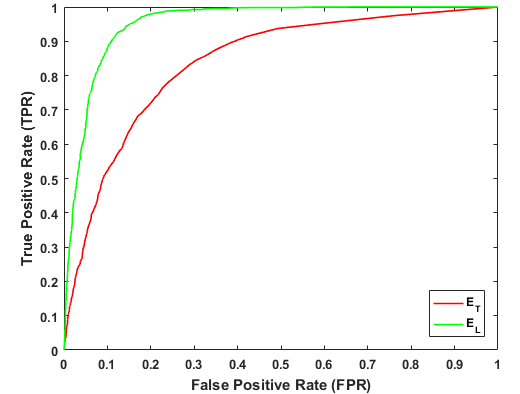
\includegraphics[width=3in, height= 1.6in]{Figures/ROC_Curve_Final}
	\caption{Receiver operator characteristics (ROC) curve of the feature $E_{T}$ and $E_{L}$, generated from BasketballDrive sequence (1080p). }
	\vspace{-1.5mm}
	\label{fig:ROC}
\end{figure}

\begin{table}[h]
	\centering
	\vspace{-2.5mm}
	\caption{The test sequence name, resolution, frame rate from the JCT-VC \cite{bossen2013common} used in this research.}
	\vspace{1.2mm}
	\renewcommand{\arraystretch}{1.3}
	\begin{tabular}{ |c|c|c| }
		\hline $\textbf{Sequence Name}$ & $\textbf{Resolution}$ & $\textbf{Frame Rate}$ \\
		\hline $BasketballPass$ & $416 \times 240$ & $50$ \\
		\hline $RaceHorses$ & $416 \times 240$ & $30$ \\
		\hline $BasketballDrive$ & $1920 \times 1080$ & $50$ \\
		\hline $Kimono$ & $1920 \times 1080$ & $24$ \\
		\hline
	\end{tabular}
	\renewcommand{\arraystretch}{1.2}
	\vspace{-5.5mm}
	\label{tab:Sequence Information}
\end{table}

\begin{figure}[t]
	\centering
	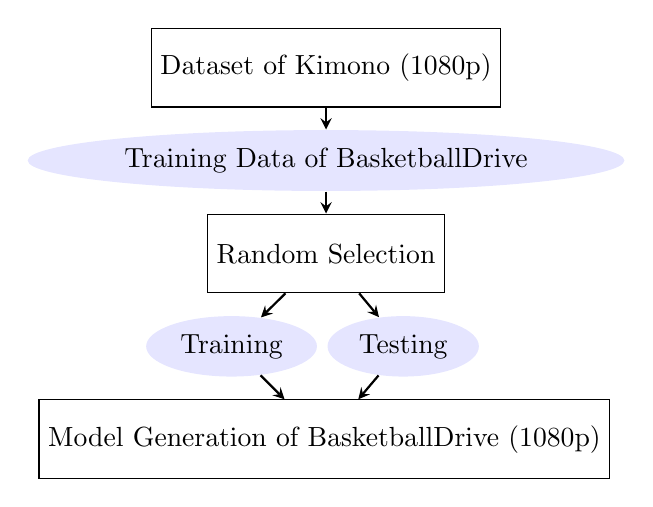
\begin{tikzpicture}[node distance=1.18cm]
	\tikzstyle{process} = [rectangle, minimum width=1cm, minimum height=1cm,text centered, draw=black, fill=white!100]
	\tikzstyle{process1} = [ellipse,fill=blue!10, minimum height=2em]
	\tikzstyle{process2} = [rectangle, minimum width=1cm, minimum height=1cm,text centered, draw=black, fill=blue!20]
	\tikzstyle{arrow} = [thick,->,>=stealth]
	
	\node (pro1) [process] {{Dataset of Kimono (1080p)}};
	\node (pro2) [process1, below of = pro1] {{Training Data of BasketballDrive}};
	\node (pro3) [process,  below of = pro2] {{Random Selection}};
	\node (pro4) [process1, below of = pro3, xshift = -1.2cm] {{Training}};
	\node (pro5) [process1, right of = pro4, xshift = 1cm] {{Testing}};
	\node (pro6) [process,  below of = pro5, xshift = -1cm] {{Model Generation of BasketballDrive (1080p)}};
	\draw [arrow] (pro1) -- (pro2);
	\draw [arrow] (pro2) -- (pro3);
	\draw [arrow] (pro3) -- (pro4);
	\draw [arrow] (pro3) -- (pro5);
	\draw [arrow] (pro4) -- (pro6);
	\draw [arrow] (pro5) -- (pro6);
	\end{tikzpicture}
	\caption{Example of Model generation for BasketballDrive sequence from the dataset of Kimono sequence.}
	\label{fig:model generation}
\end{figure}

\begin{figure}[t]
	\centering
	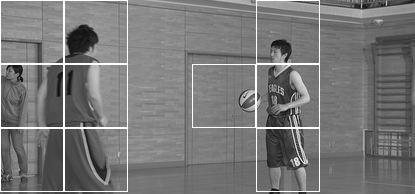
\includegraphics[width=3in, height= 1.5in]{Figures/prediction}
	\caption{Prediction of frame number 4 of BasketBallPass sequence (240p). White boundary blocks (64 $\times$ 64) are classified as multiple motion blocks by using the proposed classifier and rest of the blocks or regions are deemed to as containing single motion.}
	\vspace{-2.5mm}
	\label{fig:prediction}
\end{figure}

\begin{table*}[t]
	\centering
	\caption{Detail Experimental Results of All Test Sequence.}
	\vspace{1mm}
	\small
	\renewcommand{\arraystretch}{1.3}
	\begin{tabular}{ |c|c|c|c|c|c|c| }
		\hline $\textbf{Sequence Name}$ & $\textbf{Sensitivity (\%)}$ & $\textbf{Specificity (\%)}$ & $\textbf{Precision (\%)}$ & $\textbf{Recall (\%)}$ & $\textbf{F$_{1}$ Score (\%)}$ & $\textbf{Accuracy (\%)}$  \\
		\hline ${BasketballPass \hspace{.1cm} (240p)}$  & $91.52$ & $87.69$ & $88.13$  & $91.52$ & $89.79$ & $89.60$  \\
		\hline ${RaceHorses \hspace{.1cm} (240p)}$ & $75.78$ & $89.76$ & $74.23$  & $75.78$ & $75.00$ & $82.77$  \\
		\hline ${BasketballDrive \hspace{.1cm}(1080p)}$ & $93.95$ & $86.33$ & $87.34$  & $93.95$ & $90.53$ & $90.15$  \\
		\hline ${Kimono \hspace{.1cm} (1080p)}$  & $79.85$ & $80.26$ & $78.01$  & $79.85$ & $77.93$ & $80.05$  \\
		\hline $\textbf{Average}$ &  $\textbf{85.26}$ & $\textbf{86.01}$ & $\textbf{81.93}$ & $\textbf{85.26}$ & $\textbf{83.31}$ & $\textbf{85.64}$ \\
		\hline
	\end{tabular}
	%\renewcommand{\arraystretch}{1}
	\vspace{-3.5mm}
	\label{tab:allTable}
\end{table*}

\section{Classification Process}
\label{sec:Classification Process}

The complexity of spiting a CU or not totally, depends on how the classifier classifies the CU block more accurately. The full procedure of classification process is described in the following three subsections.

\subsection{Dataset Preprocessing}
\label{subsec:Dataset Preprocessingr}

The generated dataset has tow significant features and corresponding class label that is explained elaborately in section \ref{sec:Dataset Generation}. After examining the dataset, it is seen that the ratio of negative class and positive class tuples is 1.89, i.e. negative class has almost two times tuples than the positive class and this phenomenon is commonly called class imbalance problem. If a dataset has class imbalance problem then the output accuracy is not reliable because the the algorithm has bias problem towards the major class by applying any kind of machine learning approach. To obtain a good and reliable result class imbalance problem must be solved. The authors of  this paper used the oversampling technique for solving this issue \cite{han2011data}. Another issue regarding the dataset is that the feature values are not scaled. To speed up the classification process or to converge more rapidly, all features of the dataset are scaled up into [0,1] range.


\subsection{Classifier Selection}
\label{subsec:Decision Tree Classifier}

Decision tree is used for classifying the motion discontinuity of the blocks. The reason behind using the decision tree over SVM is that the prediction of motion discontinuity can be obtained more easily. This algorithm is often known as white box compared to other machine learning algorithms, which are referred as a black box. Breiman et al. \cite{breiman1984classification} first developed the classification and regression tree in 1984. Decision tree algorithm splits the node based on impurity or error of the node. Several split criteria are used for this algorithm. For example, gini index (GI), information gain (IG) or deviance and towing are commonly used in this purpose \cite{han2011data}. The authors of this paper used deviance for spiting a certain node and the formula of deviance or IG of a node x is as follows:  

\begin{equation}
\label{eqn_example:IG}
Deviance\hspace{0.1cm}(x) = - \sum\limits_{i} \hspace{0.1cm} p(i)\hspace{0.1cm}*\hspace{0.1cm}log \hspace{0.1cm}p(i)
\vspace{-0.1mm}
\end{equation}

Here, the sum is over the classes i at the node, and p(i) is the observed fraction of classes with class i that reach the node. A pure node has deviance 0 otherwise, it has a positive value.


\subsection{Classification}
\label{subsec:Classification}

To generate a model for classification, it is needed to train the dataset at first. For minimizing the bias problem, one sequence data is trained for testing another sequence of the same resolution. Fig. \ref{fig:model generation} shows the process, how the model is generated for BasketballDrive (1080p) sequence. Training data of BasketballDrive sequence are randomly partitioned into two categories training and testing. The authors of this paper tested three times for evaluating the model by keeping 10\%, 15\%, 20\% data respectively  for testing (i.e. cross validation dataset) and remaining data are used for training (off-line). Holdout method is used for cross-validation and pruning is used to minimize the over-fitting problem. Once the model is created for a particular sequence, then that sequence dataset is used for testing and a prediction scheme is shown in fig. \ref{fig:prediction}. The average results for various metrics that's are commonly used for classifier performance are shown in Table \ref{tab:allTable}. Similar strategy is used for other sequences for creating the model.
 

\section{Experimental Results}
\label{sec:Experimental Analysis}

The experimental section is divided into two subsections. In subsection \ref{subsec:Experimental Setup}, the experimental setup is described. Subsection \ref{subsec:Performance Analysis} gives a summary of the experimental results.

 
\subsection{Experimental Setup}
\label{subsec:Experimental Setup}
The proposed method is implemented in HEVC reference software. We used HM - 16.20 \cite{HM} for practical implementation and four QP values (22, 27, 32, 37) used to encode each sequence thats were used for experimental analysis. Low delay main GOP structure, i.e. IPPPP.....P was used as a configuration file.


\subsection{Performance Analysis}
\label{subsec:Performance Analysis}

For performance analysis, at first 50 frames of each sequence were encoded by the unmodified version of HM - 16.20 with maintaining the common test conditions of HEVC reference software \cite{bossen2013common} and the encoding results were recorded. Secondly, the same 50 frames were encoded by the proposed  HM - 16.20 encoder (modified version). The obtained two results were compared by using Bj$\o$ntrgaard delta bitrates piece-wise cubic interpolation method \cite{bjontegaard2001calculation} and in Table \ref{tab:BD Results} all encoding results are summarized.

\begin{table}[h]
	\centering
	\vspace{-2.5mm}
	\caption{Summery of encoding results.}
	\vspace{1.2mm}
	\renewcommand{\arraystretch}{1.2}
	\begin{tabular}{ |c|c|c|c| }
		\hline $\textbf{Sequence Name}$ & $\textbf{$\Delta$ Rate}$  & $\textbf{$\Delta$ Enc. Time}$ \\
		\hline $BasketballPass \hspace{.1cm} (240p)$ & $0.92\%$ & $- 43.59 \%$ \\
		\hline $RaceHorses \hspace{.1cm} (240p)$ & $1.89\%$ & $- 47.28 \%$ \\
		\hline $BasketballDrive \hspace{.1cm} (1080p)$ & $0.98\%$ & $- 42.97\%$ \\
		\hline $Kimono \hspace{.1cm} (1080p)$ & $1.73\%$ & $- 46.23\%$ \\
		\hline $\textbf{Average}$ & $\textbf{1.38\%}$ & $\textbf{-- 45.02\%}$ \\
		\hline
	\end{tabular}
	\renewcommand{\arraystretch}{1.2}
	\vspace{-6.5mm}
	\label{tab:BD Results}
\end{table}

\section{Conclusion}
\label{sec:Conclusion}
Machine learning approach plays a vital role in fast partitioning the CUs at the encoder side, when rate-distortion optimization process is invoked. In this paper, we proposed D-Tree classifier which used fruitful features for fast CU split decision to speed up the encoder. By using machine learning algorithm so-called decision tree algorithm, on average 45.02\% time complexity is reduced whereas, on average 1.38\% bit rate is increased over standalone HEVC. For BasketballPass and BasketballDrive sequences only 0.92\% and 0.98\% bit rate is increased respectively. On the other hand, 1.89\% and 1.73\% bit rate is increased for RaceHorses and Kimono sequence respectively due to having a rapid change of camera motion and illumination problem compared to other sequences and for this reason our proposed classifier performance is less compared to BasketballPass and BasketballDrive sequences. In future, we will try to increase the performance of the classifier for the test sequences.
 
\bibliographystyle{IEEEbib}
\bibliography{References_islam2021}

\end{document}
